\documentclass[11pt]{article}

%####### DON'T CHANGE MARGIN SETTINGS ###########
\newcommand{\keywordfont}{\textsc}
\newcommand{\keyword}[1]{%
  \marginpar{\raggedright\small\keywordfont{#1}}}
\reversemarginpar
\usepackage[a4paper, top=2.5cm, bottom=2.5cm, outer=2cm, inner=3.3cm, marginparwidth=72pt, heightrounded]{geometry}
%#################################

\usepackage{amsmath}
\usepackage{amssymb}
\usepackage{hyperref}
\usepackage{graphicx}
\usepackage{microtype}
\usepackage{mathtools}
\usepackage[dvipsnames]{xcolor}


\begin{document}

\Large
\begin{center}
\textbf{MA3K7 Week $10/11$ Rubric}
\\
Timothy Yap (2161367)
\end{center}
\normalsize



%--------------------------------------------------------------------------------------------------
% Pose and investigate a question inspired by the figure below.  

% Imagine posing your question to, say, an A-level student or a beginning undergraduate. Make it an interesting one!

% You can pose more than one question, but we'd prefer to see one interesting/investigative question rather than multiple easy/straightforward ones.

% Investigate the problem using the usual rubric. At this point you should try to make your rubric as complete as possible by covering most of the keywords discussed


% War Tactics

% My cousin and I used to play a game we'll call 'War Tactics'. We played this when we were very young and used 

% 1 -> 2 -> 3 -> 4 -> 5 -> 6 -> 7 -> 8 -> 9 

% What can you tell about this game?

% where we take a sequence of numbers from our grid (as in the picture) and 

%------------------------------------------------------------------------------------------------

\section{Entry} %----------------------------------------------------------------------------------

We \keyword{Problem Description} will investigate a game my cousin and I used to play. Call this game `War Tactics'. We played this when we were very young and didn't know any traditional card games. Our game began with a deck of cards and each player would take all the cards of one suit. We then fight each other by picking one card from your hand and seeing who won each`'battle'. You win the battle if you had the larger number (we thought of it as the size of your army). At the end you count how many battles you won to see who won the war, hence `War Tactics'.

Adapting this game to fit in with this week's picture. Our strategy won't be picked turn by turn but rather through a fixed sequence. For example:
\[
1 \rightarrow 2 \rightarrow 3 \rightarrow 4 \rightarrow 5 \rightarrow 6 \rightarrow 7 \rightarrow 8 \rightarrow 9
\]

As shown in our picture. All strategies will be generated by creating a path from our $3\times3$ grid of numbers. Our problem is to investigate this game of War Tactics.

We \keyword{I know} know the following:

\begin{itemize}
    \item Our game will end as there are a fix number of battles. At the end, there will either by a winner and a loser, or it will end in a draw.
    \item There are a fixed number of strategies. Fixed grid pattern with finite numbers of sequences.
    \item Playing the same sequence will always end in a draw.
\end{itemize}

We \keyword{I want} will want to answer the following questions:
\begin{itemize}
    \item What sequences are there to play?
    \item Is there an optimal strategy?
    \item What properties does this game have? 
\end{itemize}

Throughout \keyword{Introduce} this essay, we will call the first player, \textit{Player 1} and the second player, \textit{Player 2}. We denote their points with $P_1$  and $P_2$. We also introduce the term \textit{length} which is just the number of terms in our sequence. The above sequence has a length of 9. We will also have the following notation where we denote our \textit{strategy} or fixed sequence with a tuple. For example, (1, 2, 3, 4) is the strategy of playing 1, then 2, then 3, then 4. We may omit the brackets, space and commas to save space later, i.e. (1, 2, 3, 4) = 1234.

Below is an example of a full game of War Tactics.

\[
\frac{(1, 2, 3, 4, 5, 6, 7, 8, 9)}{(5, 4, 3, 2, 1, 6, 7, 8, 9)} \rightarrow (-4, -2, 0, 2, 4, 0, 0, 0, 0) \implies P_1 = 2 \text{ , } P_2 = 2 \text{ and 5 draws}
\]
We do \keyword{AHA} notice that having fixed strategies means that we don't have to consider points sequentially but rather point-wise subtraction. This saves on time as we just consider the number of positive integers as points for Player 1, the number of negative integers as points for Player 2 and any 0's as draws. Whoever has more points win and in this example, it ends in a draw.

Before \keyword{Assumptions} jumping into our attack, we state our assumptions. Generating a sequence will be done by picking any starting point on our grid and creating a sequence that goes through all numbers. We will only allow our sequence to move to the next grid point vertically or horizontally, so no diagonal movements. This is a possible expansion for our Review. Our last assumption is that both players want to win and will play optimally. 



%--------------------------------------------------------------------------------------------------

\section{Attack} %----------------------------------------------------------------------------------

We begin \keyword{Strategic Specialisation} by reducing our problem to games of length 4, with sequences generated by using the top-right $2 \times 2$ sub-grid. We have 8 sequences as starting at each corner, we have two options to follow. This is shown below.

\[
\begin{bmatrix}
4 & \leftarrow & 3\\
 & & \uparrow \\
1 & \rightarrow & 2
\end{bmatrix}\hspace{25pt}
\begin{bmatrix}
4 & \rightarrow & 3\\
\uparrow & & \downarrow \\
1 & & 2
\end{bmatrix}\hspace{25pt}
\begin{bmatrix}
4 & \rightarrow & 3\\
 \uparrow & &\\
1 & \leftarrow & 2
\end{bmatrix}\hspace{25pt}
\begin{bmatrix}
4 & \leftarrow & 3\\
\downarrow & &\uparrow \\
1 & & 2
\end{bmatrix}\vspace{5pt}
\]
\[
\begin{bmatrix}
4 & \leftarrow & 3\\
\downarrow & & \\
1 & \rightarrow & 2
\end{bmatrix}\hspace{25pt}
\begin{bmatrix}
4 &  & 3\\
\uparrow & & \downarrow \\
1 & \leftarrow & 2
\end{bmatrix}\hspace{25pt}
\begin{bmatrix}
4 & \rightarrow & 3\\
 & & \downarrow \\
1 & \leftarrow & 2
\end{bmatrix}\hspace{25pt}
\begin{bmatrix}
4 &  & 3\\
\downarrow & & \uparrow \\
1 & \rightarrow & 2
\end{bmatrix}
\]
We utilised a lot of symmetry \keyword{AHA} which hopefully will carry to the $3 \times 3$ grid. We now try \keyword{Try} to match each strategy against each other. With Player 1 playing the strategies on the left column against Player 2 playing strategies from the top row. We show the points in a tuple form $(P_1, P_2, X)$.With $P_1$ and $P_2$ as defined above and $X$ as whether Player 1 won or lost, i.e. $W$ for a win and $L$ for a loss. We will write $D$ to indicate a draw.


\begin{table}[h]
    \centering
    \begin{tabular}{ccccccccc}
  Player 1's& \multicolumn{8}{c}{Player 2's Strategies}\\
          Strategies&  1234&  1432&  2143&  2341&  3412&  3214&  4321& 4123\\
1234& $( 0 , 0 , \textcolor{blue}{D})$
& $( 1 , 1 , \textcolor{blue}{D})$
& $( 2 , 2 , \textcolor{blue}{D})$
& $( 1 , 3 , \textcolor{Red}{L})$
& $( 2 , 2 , \textcolor{blue}{D})$
& $( 1 , 1 , \textcolor{blue}{D})$
& $( 2 , 2 , \textcolor{blue}{D})$
& $( 3 , 1 , \textcolor{Green}{W})$
\\
          1432& $( 1 , 1 , \textcolor{blue}{D})$
& $( 0 , 0 , \textcolor{blue}{D})$
& $( 1 , 3 , \textcolor{Red}{L})$
& $( 2 , 2 , \textcolor{blue}{D})$
& $( 1 , 1 , \textcolor{blue}{D})$
& $( 2 , 2 , \textcolor{blue}{D})$
& $( 3 , 1 , \textcolor{Green}{W})$
& $( 2 , 2 , \textcolor{blue}{D})$
\\
          2143& $( 2 , 2 , \textcolor{blue}{D})$
& $( 3 , 1 , \textcolor{Green}{W})$
& $( 0 , 0 , \textcolor{blue}{D})$
& $( 1 , 1 , \textcolor{blue}{D})$
& $( 2 , 2 , \textcolor{blue}{D})$
& $( 1 , 3 , \textcolor{Red}{L})$
& $( 2 , 2 , \textcolor{blue}{D})$
& $( 1 , 1 , \textcolor{blue}{D})$
\\
          2341& $( 3 , 1 , \textcolor{Green}{W})$
& $( 2 , 2 , \textcolor{blue}{D})$
& $( 1 , 1 , \textcolor{blue}{D})$
& $( 0 , 0 , \textcolor{blue}{D})$
& $( 1 , 3 , \textcolor{Red}{L})$
& $( 2 , 2 , \textcolor{blue}{D})$
& $( 1 , 1 , \textcolor{blue}{D})$
& $( 2 , 2 , \textcolor{blue}{D})$
\\
          3412& $( 2 , 2 , \textcolor{blue}{D})$
& $( 1 , 1 , \textcolor{blue}{D})$
& $( 2 , 2 , \textcolor{blue}{D})$
& $( 3 , 1 , \textcolor{Green}{W})$
& $( 0 , 0 , \textcolor{blue}{D})$
& $( 1 , 1 , \textcolor{blue}{D})$
& $( 2 , 2 , \textcolor{blue}{D})$
& $( 1 , 3 , \textcolor{Red}{L})$
\\
          3214& $( 1 , 1 , \textcolor{blue}{D})$
& $( 2 , 2 , \textcolor{blue}{D})$
& $( 3 , 1 , \textcolor{Green}{W})$
& $( 2 , 2 , \textcolor{blue}{D})$
& $( 1 , 1 , \textcolor{blue}{D})$
& $( 0 , 0 , \textcolor{blue}{D})$
& $( 1 , 3 , \textcolor{Red}{L})$
& $( 2 , 2 , \textcolor{blue}{D})$
\\
          4321& $( 2 , 2 , \textcolor{blue}{D})$
& $( 1 , 3 , \textcolor{Red}{L})$
& $( 2 , 2 , \textcolor{blue}{D})$
& $( 1 , 1 , \textcolor{blue}{D})$
& $( 2 , 2 , \textcolor{blue}{D})$
& $( 3 , 1 , \textcolor{Green}{W})$
& $( 0 , 0 , \textcolor{blue}{D})$
& $( 1 , 1 , \textcolor{blue}{D})$
\\
          4123& $( 1 , 3 , \textcolor{Red}{L})$
& $( 2 , 2 , \textcolor{blue}{D})$
& $( 1 , 1 , \textcolor{blue}{D})$
& $( 2 , 2 , \textcolor{blue}{D})$
& $( 3 , 1 , \textcolor{Green}{W})$
& $( 2 , 2 , \textcolor{blue}{D})$
& $( 1 , 1 , \textcolor{blue}{D})$
& $( 0 , 0 , \textcolor{blue}{D})$
\\
    \end{tabular}
    \caption{War Tactics for Strategies of length 4}
    \label{tab:my_label}
\end{table}
We see \keyword{Check}  that when Player 1 and 2 play the same strategy, we correctly get $(0, 0 ,D)$. This is shown on the diagonal. Analysing our table, we observe that each strategy that Player 1 plays has a counter strategy and is a counter strategy to one of Player  2's strategy. In all other cases, we end in a draw. We also note that a player can only win a maximum of 3 battles, and in order to win, they need to win exactly 3 games. The one lost battle always comes from one of the battles being with a 1. With our table being symmetric, we conjecture the following:

The optimal strategy \keyword{Conjecture} is to play each possible strategy randomly with each strategy given a $\frac{1}{8}$ probability of being picked.

We \keyword{Justify} justify this as this is similar to Rock, Paper, Scissors which a zero-sum game without perfect information. War Tactics played with length 4 sequences is clearly a zero-sum game which means if one player wins, the other loses. It also has imperfect information which states that we know what actions the other player may play and their payoff, but not their exact choice. Any strategy that prioritises one sequence over the others will give the advantage to their opponent as they may play the corresponding counter strategy more often. This is explored in my related module ST234: Games and Decisions. In said module, we calculated that the probabilities of playing any move in Rock, Paper, Scissors is $\frac{1}{3}$ by setting each move as $p_1$, $p_2$ and $1 - p_1 - p_2$ respectively. If we did the same, we would find that all probabilities would equal  $\frac{1}{8}$. 

We also check \keyword{Check} this in Python by simulating many games and finding the average win/loss ratio. We found that we get an approximately 50\% of winning with our random strategy which is expected given our zero-sum game. We simulated 100 million games and had an exact solution of 0.50000853. 

Moving to our $3 \times 3$ grid, we now generate sequences of length 9. To begin our attack on our more advanced version of War Tactics, we start by investigating the possible sequences generated from our grid. We \keyword{Try} attempt some by hand, keeping in mind symmetry of grid, and we begin to notice certain patterns. We find and \textbf{conjecture}\keyword{Conjecture}\textbf{ there are 40 unique sequences.} We will go through three following cases, where we start in the middle, at the middle of each side, or the corner.
\\ \textbf{Case 1} -\keyword{Justify} Let's begin our sequence from the middle, at 1. We find that we can go to the following 4 numbers, namely, 2, 4, 6, and 8. This is shown below in our first grid. With symmetry, we just take 2 as our example (shown with $\Rightarrow$). At each number we can loop around two different ways, either up or down. We go up in our example. This gives us a total of 8 unique sequences when starting at the middle. 
\[
\begin{bmatrix}
5 & & 4 & & 3\\
 & & \uparrow & & \\
6 & \leftarrow & 1 & \Rightarrow & 2\\
 & & \downarrow & & \\
7 & & 8 & & 9\\
\end{bmatrix} \implies
\begin{bmatrix}
5 & \ \ & 4 & \ \ & 3\\
 & &  & & \Uparrow \\
6 & & 1 & \Rightarrow & 2\\
 & &  & & \downarrow \\
7 & & 8 & & 9\\
\end{bmatrix} \implies
\begin{bmatrix}
5 & \leftarrow & 4 & \leftarrow & 3\\
\downarrow & &  & & \uparrow\\
6 & & 1 & \rightarrow & 2\\
\downarrow & &  & & \\
7 & \rightarrow & 8 & \rightarrow & 9\\
\end{bmatrix}
\]
\\ \textbf{Case 2} -\keyword{Justify} Let's begin at any middle of each side, i.e. 2, 4, 6, or 8. We can use symmetry and just take 6 as our starting point. We can go to three different numbers, but only two different type of points, the middle or the corners. In the first sub-case, we find that there will always be some \keyword{Stuck}numbers that cannot be in our sequence. 
\[
\begin{bmatrix}
5 & & 4 &  \ \  & 3\\
\uparrow & & & & \\
6 & \Rightarrow & 1 & & 2\\
\downarrow & &  & & \\
7 & & 8 & & 9\\
\end{bmatrix} \implies
\begin{bmatrix}
5 & \ \ & 4 & & 3\\
 & & \Uparrow & & \\
6 & \Rightarrow & 1 & \rightarrow & 2\\
 & & \downarrow & &  \\
7 & & 8 &  & 9\\
\end{bmatrix} \implies
\begin{bmatrix}
\textcolor{blue}{5} & \ \ & 4 & \rightarrow & 3\\
 & & \uparrow & & \downarrow \\
6 & \rightarrow & 1 & & 2\\
 & &  & & \downarrow \\
7 & \leftarrow & 8 & \leftarrow & 9\\
\end{bmatrix}
\]
\[
\begin{bmatrix}
5 & & 4 &  \ \  & 3\\
\Uparrow & & & & \\
6 & \rightarrow & 1 & & 2\\
\downarrow & &  & & \\
7 & & 8 & & 9\\
\end{bmatrix} \implies
\begin{bmatrix}
5 & \Rightarrow & 4 &  \ \  & 3\\
\Uparrow & & & & \\
6 &  & 1 & & 2\\
 & &  & & \\
7 & & 8 & & 9\\
\end{bmatrix} \implies
\begin{bmatrix}
5 & \Rightarrow & 4 & \rightarrow & 3\\
\Uparrow & & & & \downarrow \\
6 & & \textcolor{blue}{1} & & 2\\
 & &  & & \downarrow \\
7 & \leftarrow & 8 & \leftarrow & 9\\
\end{bmatrix}
\]
When exploring the other different sequences, we find that no \keyword{AHA}sequences can exist when starting at any of 2, 4, 6, or 8.
\\ \textbf{Case 3} -\keyword{Justify} Lastly, we start at the corners, i.e. 3, 5, 7, or 9. We can also use symmetry and just take 5 as our starting point. At each corner, we will have one up/down and one left/right option, leaving us with 2 choices at each corner. Again, with symmetry we just go down to 6. We now split off into two sub-cases; 1) going to the centre, or 2) making a straight row/column. In our first sub-case we see that there is only one possible sequence.
\[
\begin{bmatrix}
5 & \rightarrow & 4 & & 3\\
\Downarrow  & & & & \\
6 & & 1 & & 2\\
  & &  & & \\
7 & & 8 & & 9\\
\end{bmatrix} \implies
\begin{bmatrix}
5 & & 4 & & 3\\
\Downarrow  & & & & \\
6 & \Rightarrow & 1 & & 2\\
\downarrow  & &  & & \\
7 & & 8 & & 9\\
\end{bmatrix} \implies
\begin{bmatrix}
5 & & 4 & \rightarrow & 3\\
\downarrow & & \uparrow & & \downarrow \\
6 & \rightarrow & 1 & & 2\\
 & &  & & \downarrow \\
7 & \leftarrow & 8 & \leftarrow & 9\\
\end{bmatrix}
\]
We now move \keyword{Justify}on to 2), the straight column case. In this case we must exit the corner to the only option, in this example, it goes from 7 to 8. Now we have 2 sub-sub-cases; a) going up to the centre, or b) going into the corner and making a large L. We begin by exploring a). We only have one option; that is to make an 'S' looking sequence. 
\[
\begin{bmatrix}
5 & & 4 & & 3\\
\Downarrow  & & & & \\
6 & & 1 & & 2\\
\Downarrow & & \uparrow & & \\
7 & \Rightarrow & 8 & \rightarrow & 9\\
\end{bmatrix} \implies
\begin{bmatrix}
5 & & 4 & & 3\\
\Downarrow  & & & & \\
6 & & 1 & & 2\\
\Downarrow & & \Uparrow & & \\
7 & \Rightarrow & 8 & \rightarrow & 9\\
\end{bmatrix} \implies
\begin{bmatrix}
5 & & 4 & \rightarrow & 3\\
\downarrow & & \uparrow & & \downarrow \\
6 & & 1 & & 2\\
\downarrow & & \uparrow & & \downarrow \\
7 & \rightarrow & 8 & & 9\\
\end{bmatrix}
\]
We now move \keyword{Justify}to b), where we get a further two sub-cases; i) we go to the centre, or ii) we go around the centre. These give us two options when reaching sub-sub-case b).
\[
\begin{bmatrix}
5 & & 4 & & 3\\
\Downarrow  & & & & \\
6 & & 1 & & 2\\
\Downarrow & & \uparrow & & \\
7 & \Rightarrow & 8 & \Rightarrow & 9\\
\end{bmatrix} \implies
\begin{bmatrix}
5 & & 4 & \rightarrow & 3\\
\downarrow  & & \uparrow & & \\
6 & & 1 & \leftarrow & 2\\
\downarrow & &  & & \uparrow \\
7 & \rightarrow & 8 & \rightarrow & 9\\
\end{bmatrix} \text{     or     }
\begin{bmatrix}
5 & & 4 & \leftarrow & 3\\
\downarrow  & & \downarrow & & \uparrow \\
6 & & 1 & & 2\\
\downarrow & &  & & \uparrow \\
7 & \rightarrow & 8 & \rightarrow & 9\\
\end{bmatrix}
\]
Adding up all our \keyword{Check}cases, we get 8 sequence when starting at the middle and $4 \times 2(1 + 3) = 32$ cases when starting at a corner. The first 4 term comes from four corners and the 2 coefficient comes from each corner having two choices. In sub-case 1), we only have 1 option and in sub-case 2) we get 3 options. Thus we have a total of 40 potential sequences. 

By comparing each \keyword{Try}sequence against one another, we obtain the following results below. A draw is represent by a 0, a win for Player 1 is represented by a green 1, and a loss for Player 1 is represented by a red -1.

\begin{figure}[h]
   \centering
   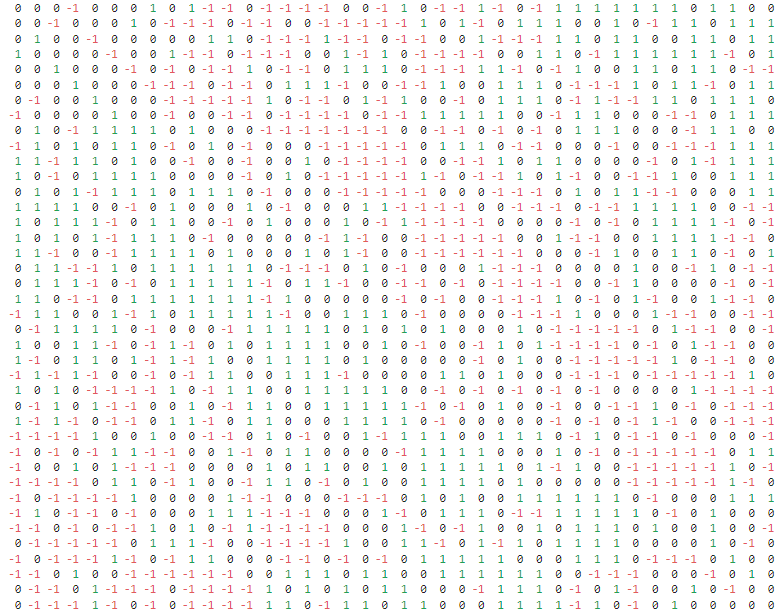
\includegraphics[width=6.15in]{beautiful.PNG}
   \label{myfig}
\end{figure}

From our observation, we find that our resulting table is symmetric along the diagonal when looking at draws. It is reflected along said diagonal and multiplied by minus -1. It is \keyword{Ooo} difficult to explain but this almost looks like art. Seemingly random. This does depend on how I ordered the strategies but this was done by sorting smallest to largest. We may find it difficult \keyword{Stuck} to determine an optimal strategy when looking a this. But when \keyword{Check} using Python, a random strategy does give an approximate 50\% ratio. Again this was tested with 100 million simulations.

%---------------------------------------------------------------------------------------------------

\section{Review} %----------------------------------------------------------------------------------

To \keyword{Check} answer our initial questions, we found that there are exactly 40 unique sequences that can be generated under our assumptions. When justifying our conjecture, we gave each case which can generate all possible sequences one may play. Furthermore, we found that this game is analogous to Rock, Paper, Scissors where a randomised strategy is best. However, this may not be the case as some rows have more wins than losses. This may allude to some strategies have better odds. However, those probabilities are likely close enough that a randomised strategy is close to optimal. This game has the following properties; all players have the same options, there is imperfect information, and the pay off matrix (this would be the $X$ value in Table 1) is symmetric. Fully solving this game would definitely go beyond the scope of this essay.

Finding \keyword{Reflect} a question was difficult. Getting the right balance of being difficult enough to properly explore different aspects of math while being accessible enough to find interesting answers. Hopefully, I was able to do so. I initially had a question of what kinds of passwords could be created, exactly what I found when generating sequences. I realised that would have been slightly too easy of a question. I'm glad to have incorporated something from my childhood into the question. 

Besides the \keyword{Reflect} challenge of coming up with a suitable question, I found the use of Python to be a lot harder when generating sequences. However, it was able to quickly calculate a vast number of games. This help produce both tables of results. Overall I would say I'm most proud of my figure, even though I don't fully grasp what it entails. 

There are various ways to \keyword{Extend} extend the game. Here are some ideas of how to do so:
\begin{itemize}
    \item Different ways to generate sequences: Allow any sequence of number, any combination of 1, 2, \dots , 8, 9. Move away from these numbers and allow any allocation of resources.
    \item Instead of a simple `battle' of highest card wins, you could;
    \begin{itemize}
        \item Have the winner add the opponent's card and divide by two. Use this new card to play the next turn
        \item Have the winner add the opponent's card modulo 10, or any other number.
    \end{itemize}
\end{itemize}

A quick example of extending \keyword{Extend} our game by adding and dividing by two:
\[
\frac{(1,3,2) }{(3,1,2)} \xrightarrow[P_1 = 0, P_2 = 1]{(1 + 3)/2 =2} \frac{(3,2) }{(2,1,2)} \xrightarrow[P_1 = 1, P_2 = 1]{(3 + 2)/2 =2.5}
\frac{(2.5,2) }{(1,2)} \xrightarrow[P_1 = 2, P_2 = 1]{(2.5 + 1)/2 =1.75}
\frac{(1.75,2)}{(2)} \xrightarrow[P_1 = 2, P_2 = 2]{(1.75 + 2)/2 =1.875} 
\frac{(2)}{(1.875)}
\]
And the winner is Player 1 with 3 points! Maybe one day I could play this with my cousin.

\section*{Supplementary material}
The code for this assignment can be found on my GitHub page:  \url{https://github.com/LazyTim/MA3K7/blob/main/MA3K7%20-%20Assignment%205.ipynb}.


\end{document}